\begin{figure*}
	\center{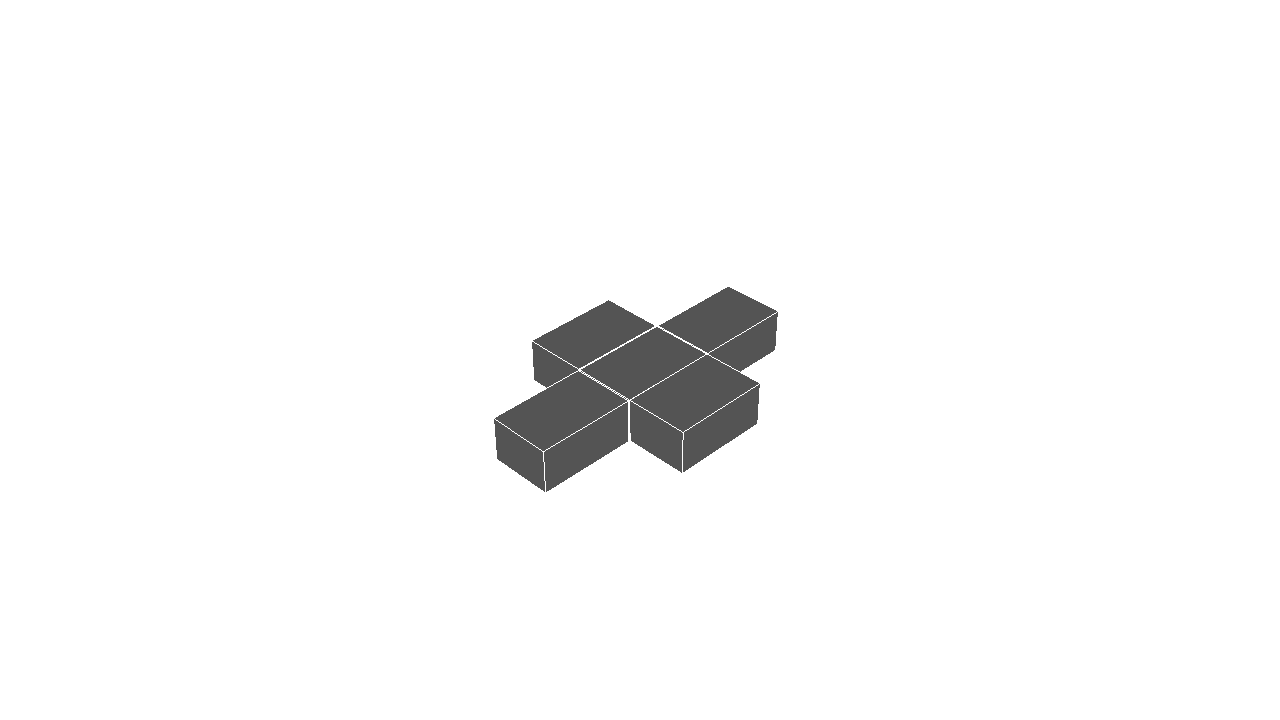
\includegraphics[width=0.5\linewidth]{img/caps/test0_1.png}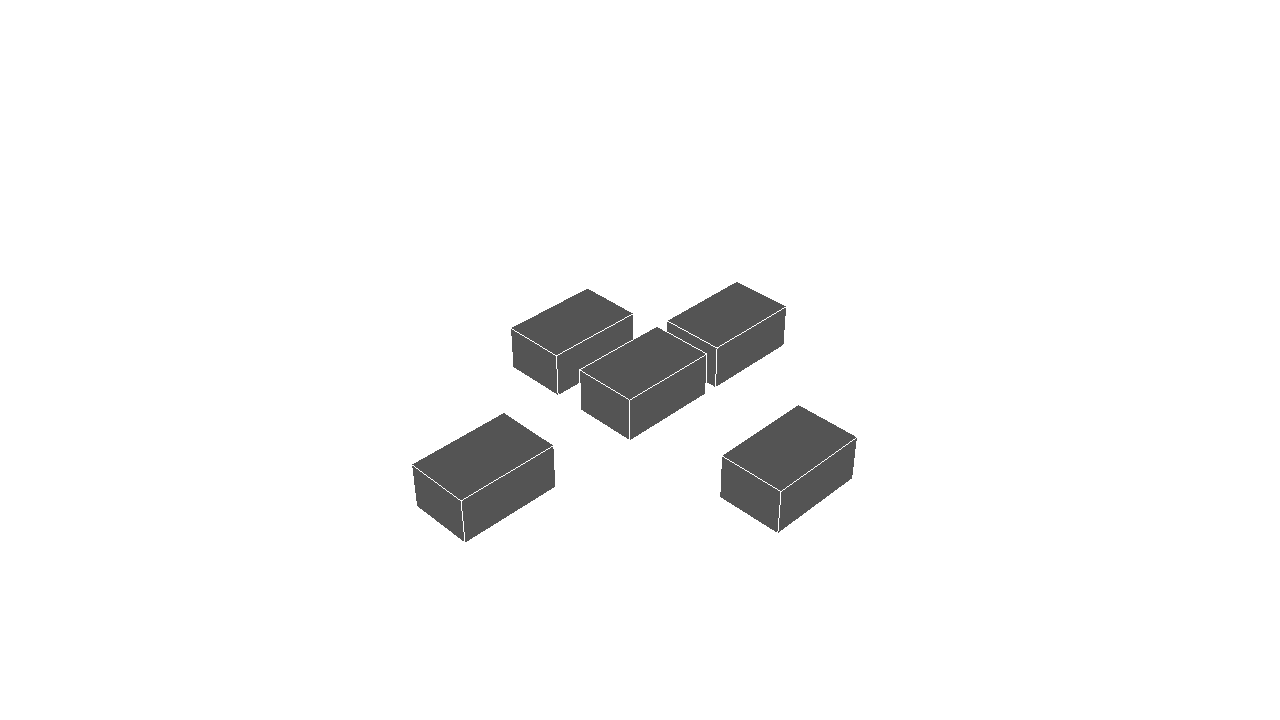
\includegraphics[width=0.5\linewidth]{img/caps/test0_2.png}}
	\caption{\label{fig:test0} Modelo 1 antes e depois da explos�o da parte central.}
\end{figure*}

\begin{figure*}
	\center{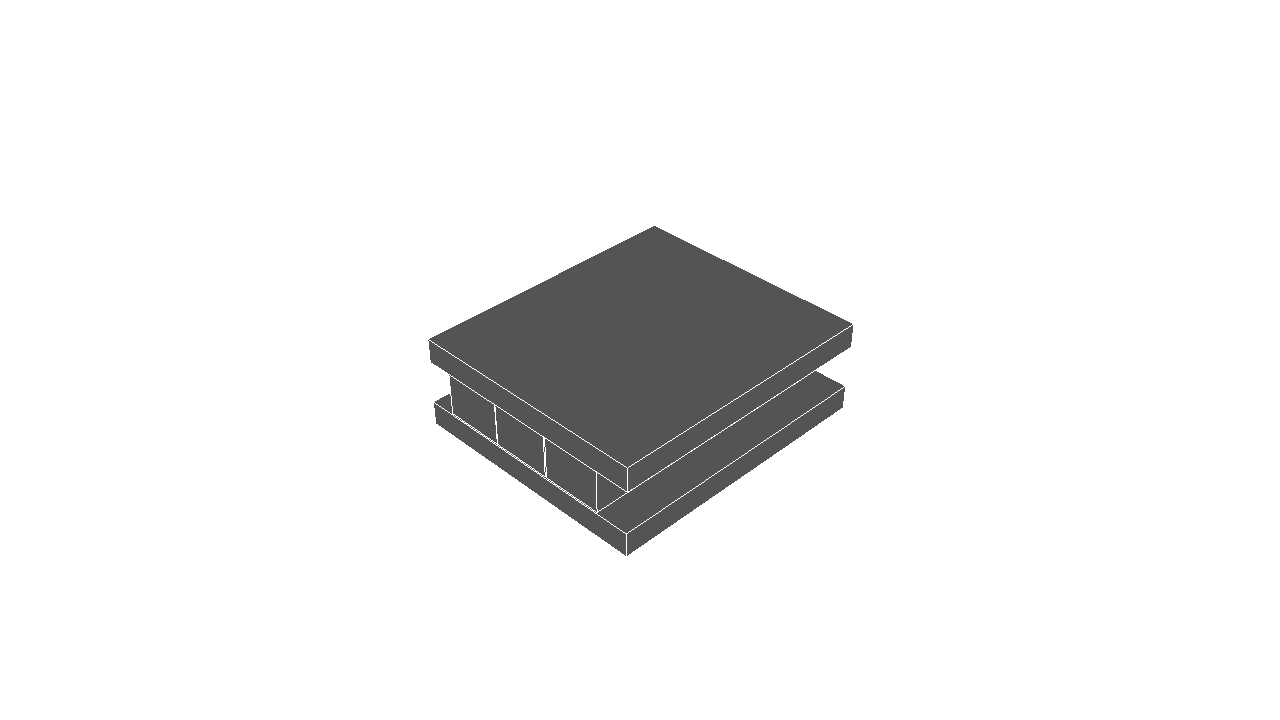
\includegraphics[width=0.3\linewidth]{img/caps/test1_1.png}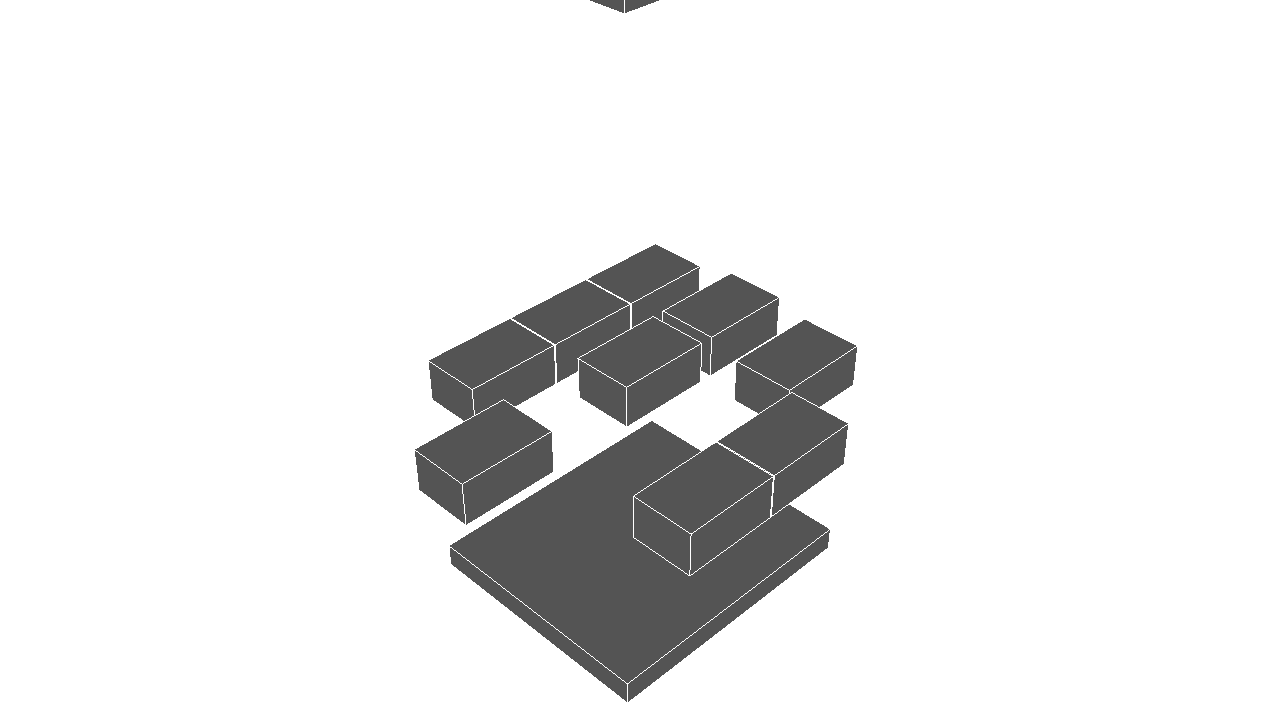
\includegraphics[width=0.3\linewidth]{img/caps/test1_2.png}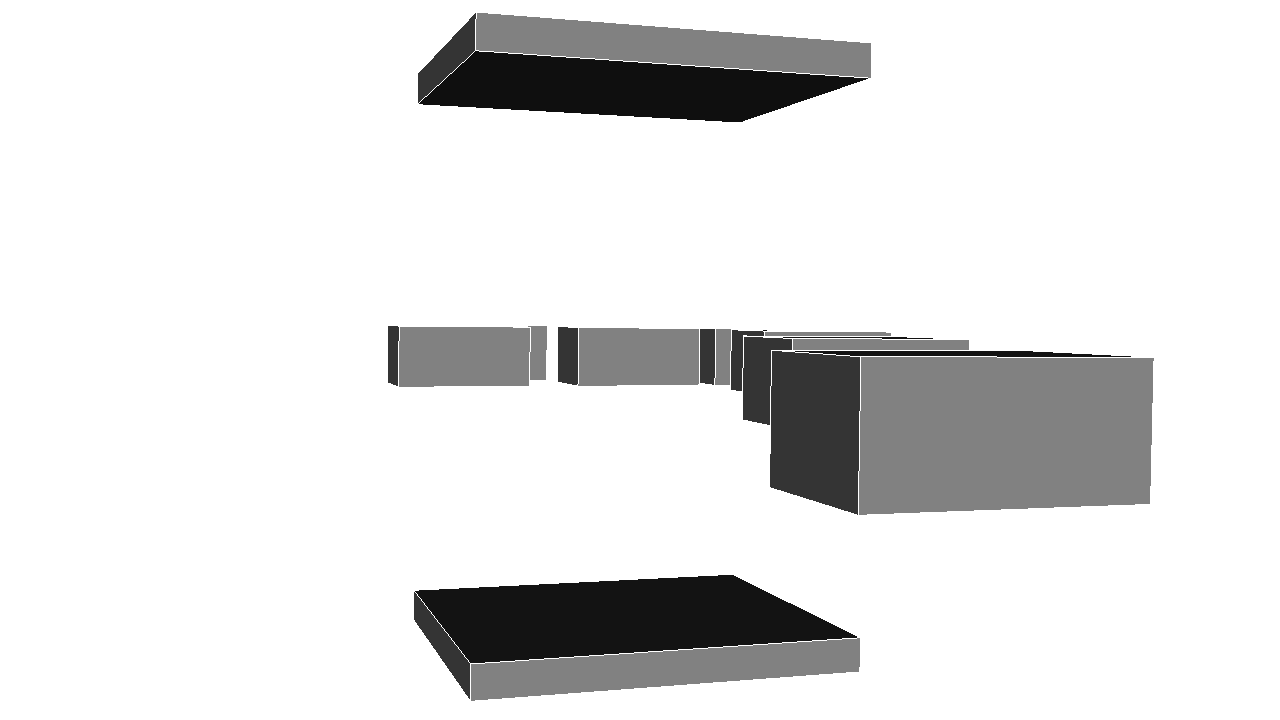
\includegraphics[width=0.3\linewidth]{img/caps/test1_3.png}}
	\caption{\label{fig:test1} Modelo 2 antes e depois da explos�o da parte central, e alterando a posi��o da c�mera.}
\end{figure*}

\begin{figure*}
	\center{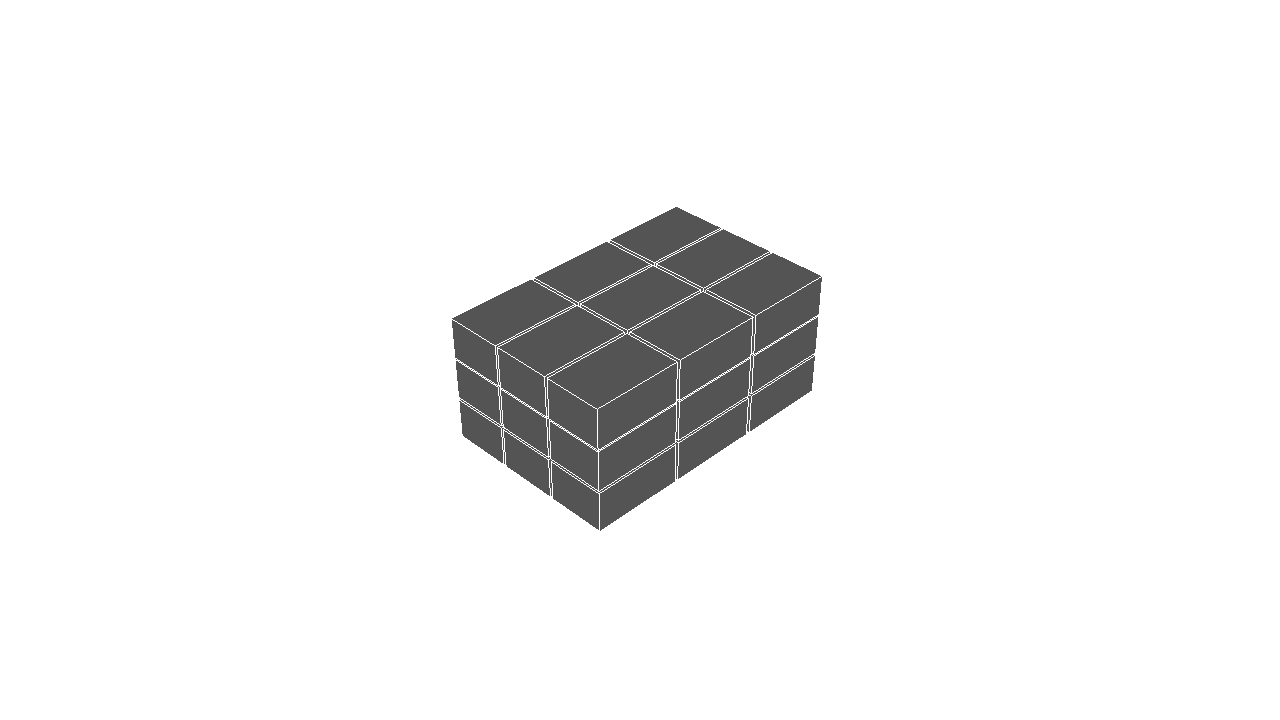
\includegraphics[width=0.5\linewidth]{img/caps/test2_1.png}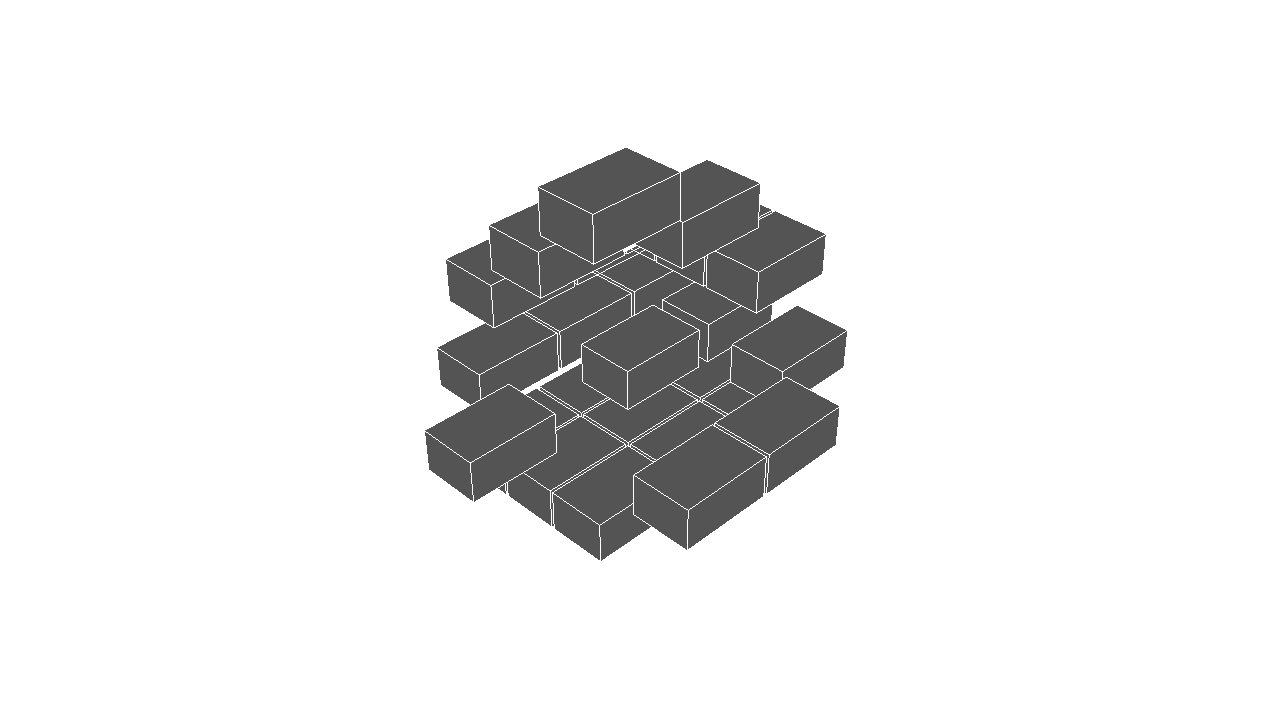
\includegraphics[width=0.5\linewidth]{img/caps/test2_2.png}\\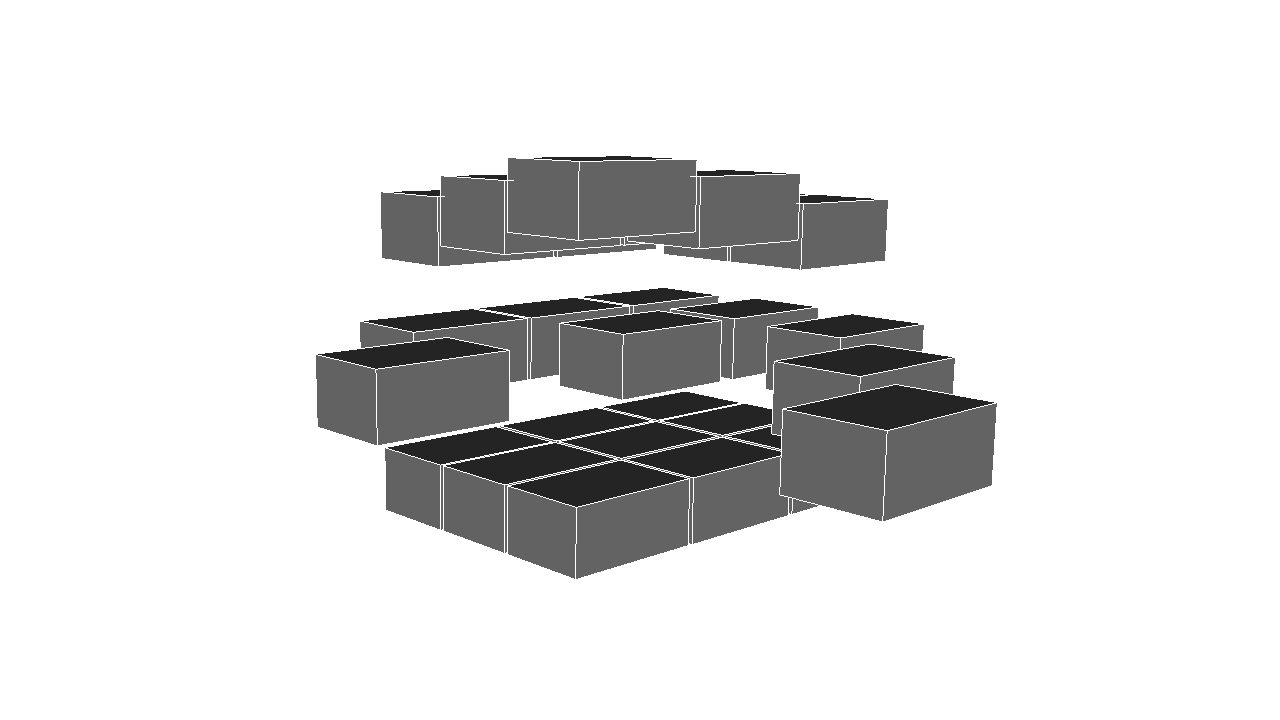
\includegraphics[width=0.5\linewidth]{img/caps/test2_3.png}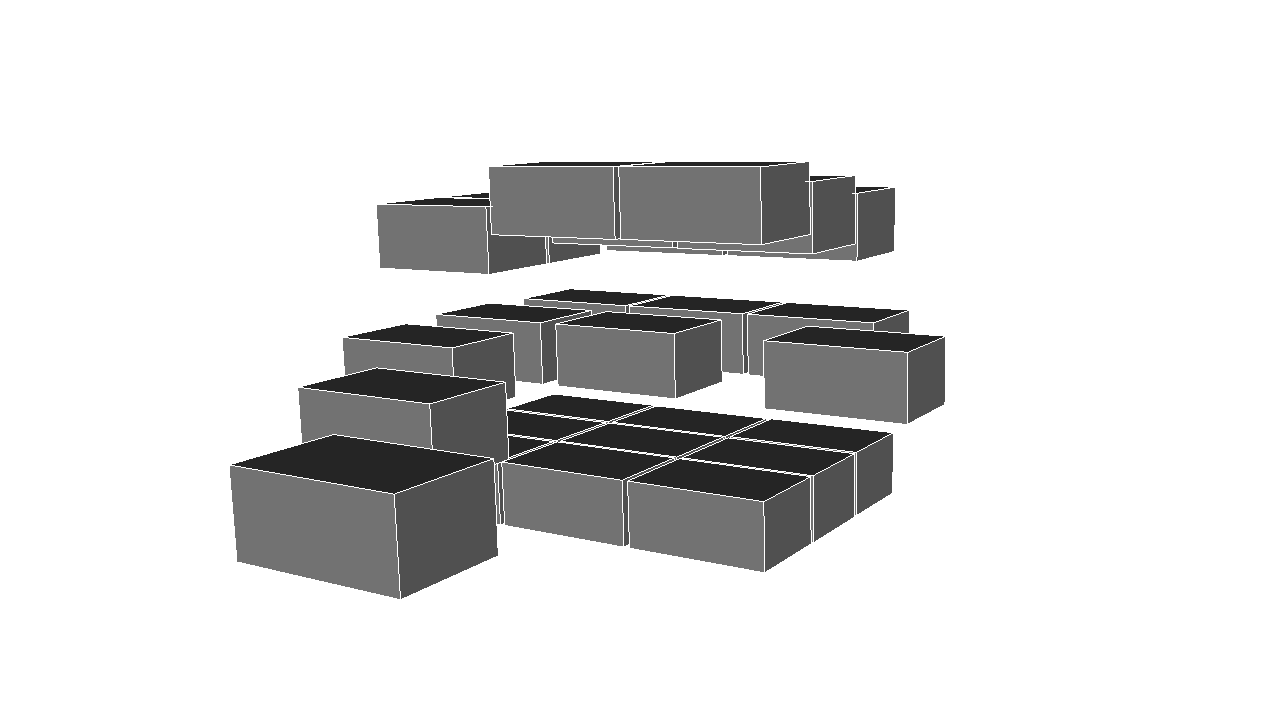
\includegraphics[width=0.5\linewidth]{img/caps/test2_4.png}}
	\caption{\label{fig:test2} Modelo 3 antes e depois da explos�o da parte central, e alterando a posi��o da c�mera.}
\end{figure*}

\begin{figure*}
	\center{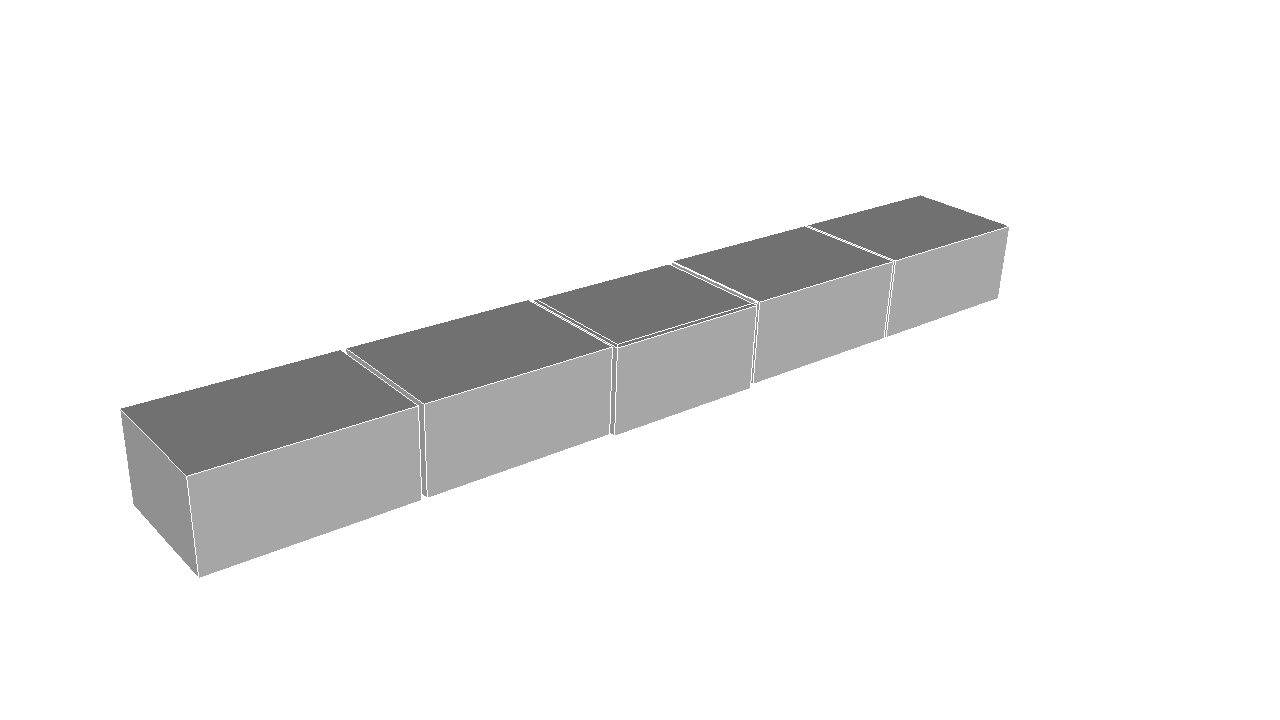
\includegraphics[width=0.5\linewidth]{img/caps/test4_1.png}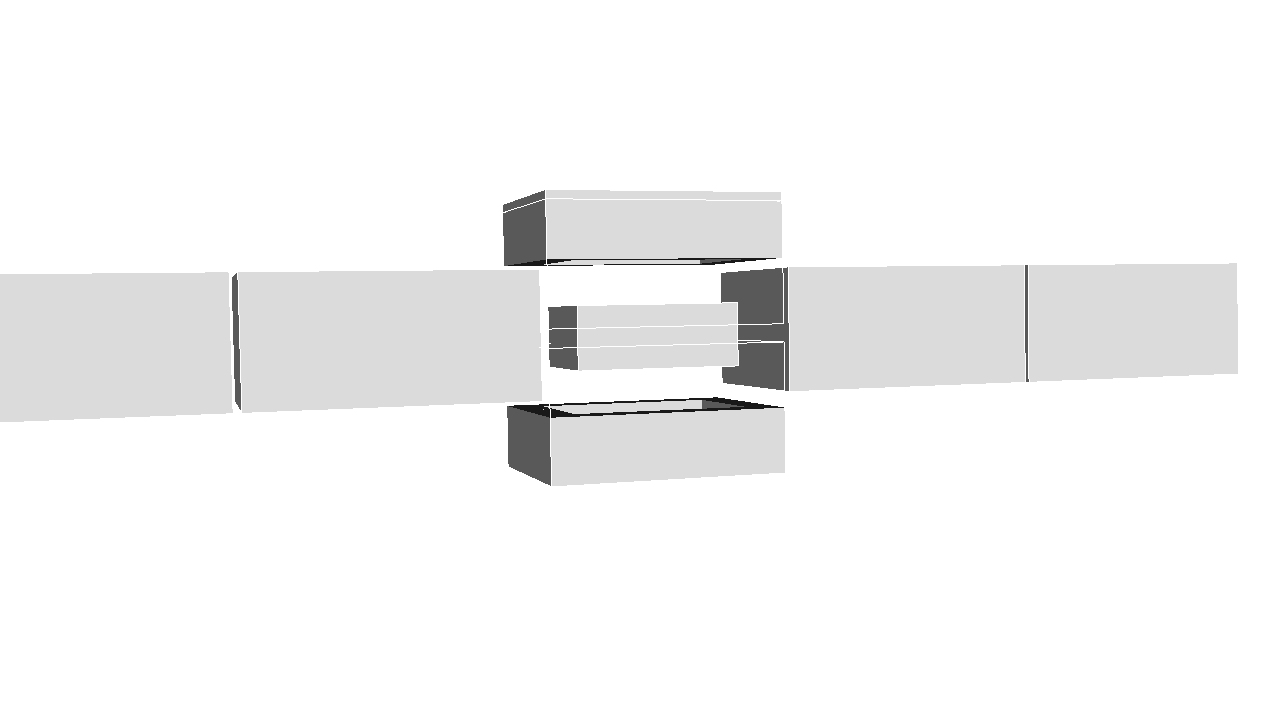
\includegraphics[width=0.5\linewidth]{img/caps/test4_2.png}\\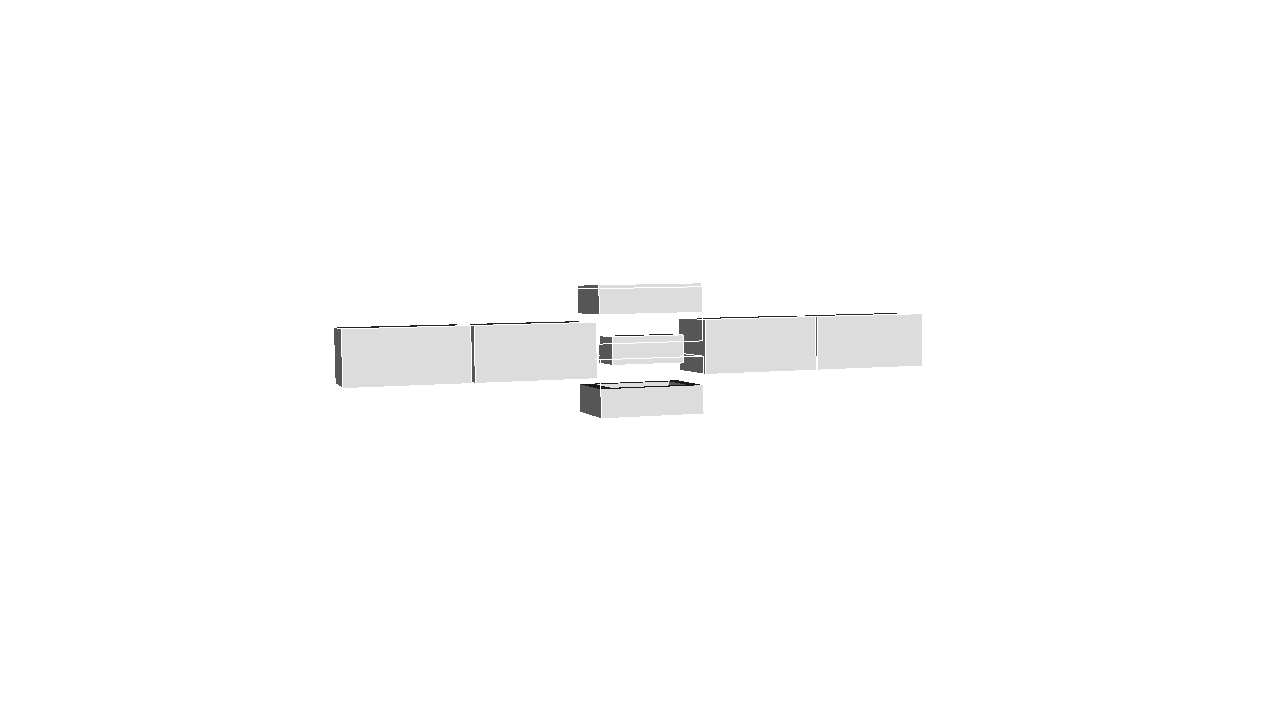
\includegraphics[width=0.5\linewidth]{img/caps/test4_3.png}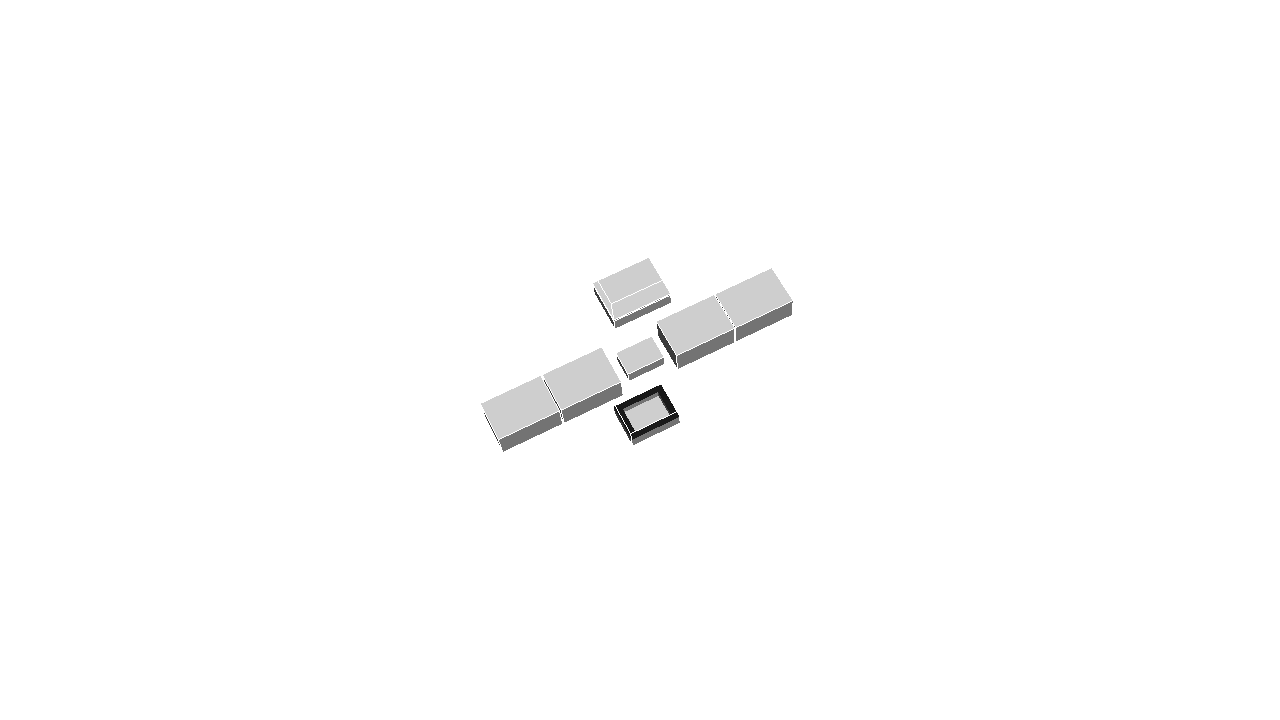
\includegraphics[width=0.5\linewidth]{img/caps/test4_4.png}}
	\caption{\label{fig:test4} Modelo 4 antes e depois da explos�o da parte central, com uma parte envolvendo totalmente outra parte.}
\end{figure*}


\begin{figure*}
	\center{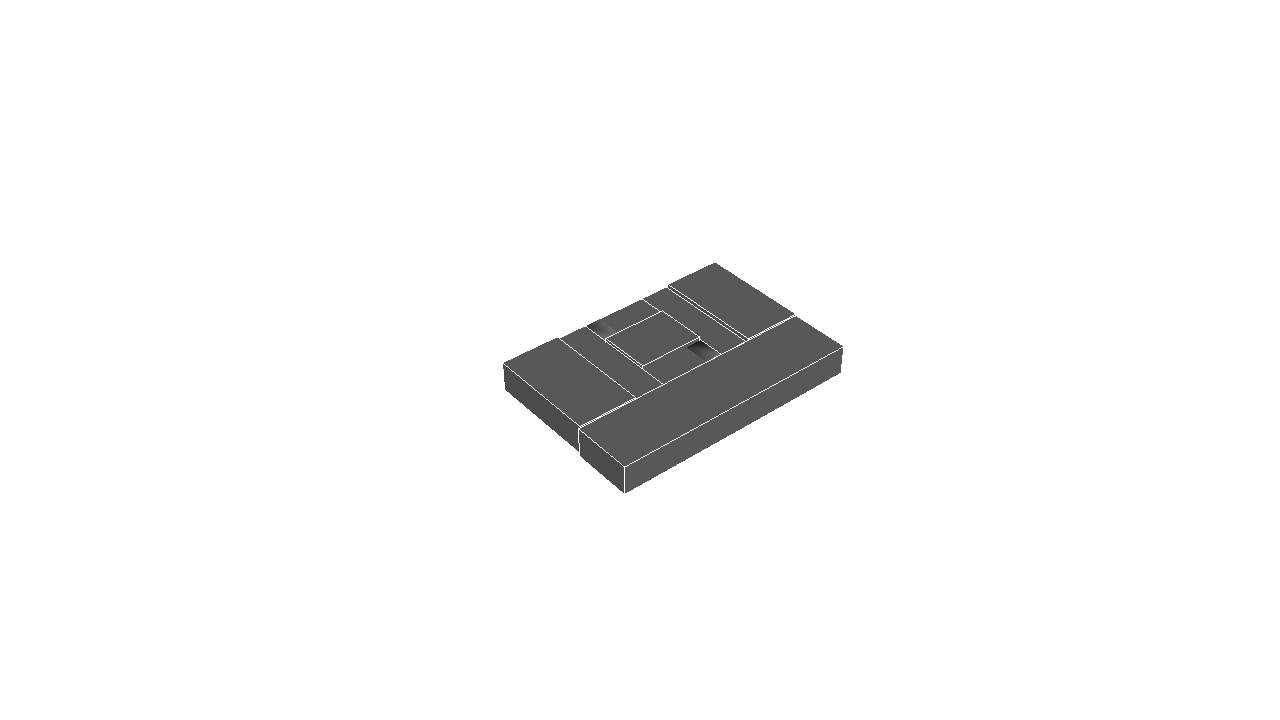
\includegraphics[width=0.5\linewidth]{img/caps/test9_1.png}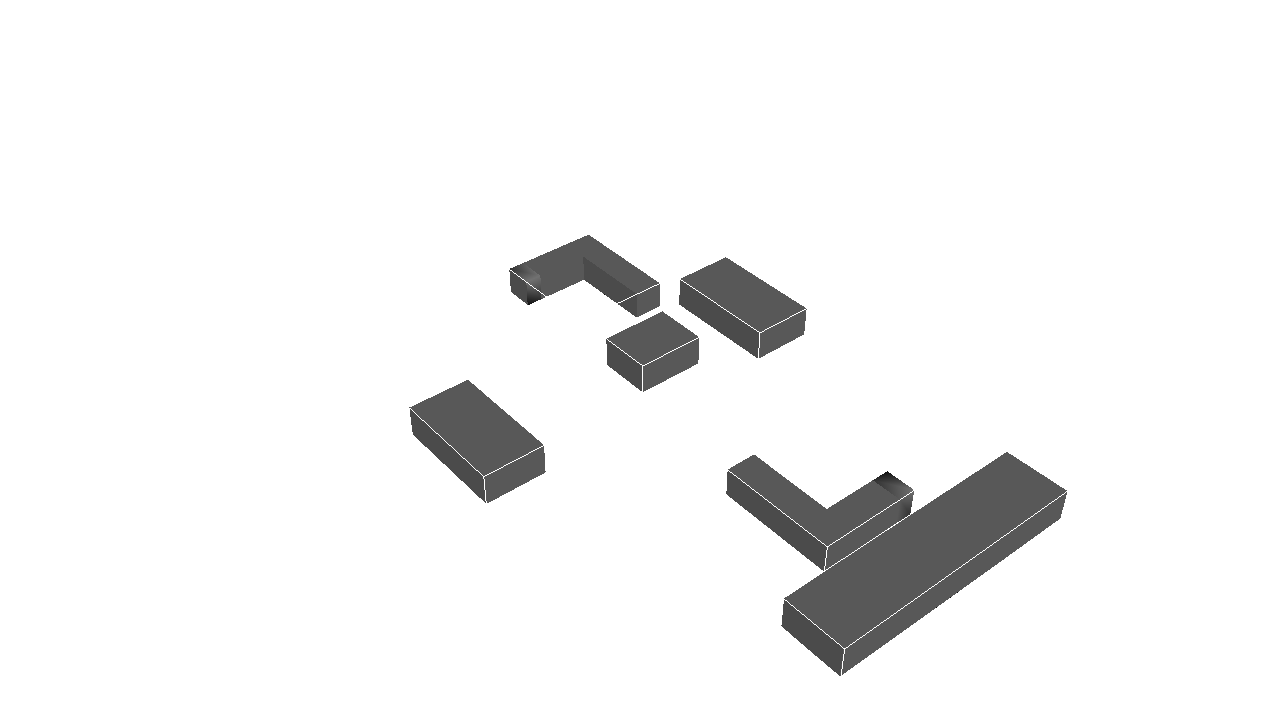
\includegraphics[width=0.5\linewidth]{img/caps/test9_2.png}}
	\caption{\label{fig:test9} Modelo 5 antes e depois da explos�o da parte central.}
\end{figure*}

\begin{figure*}
	\center{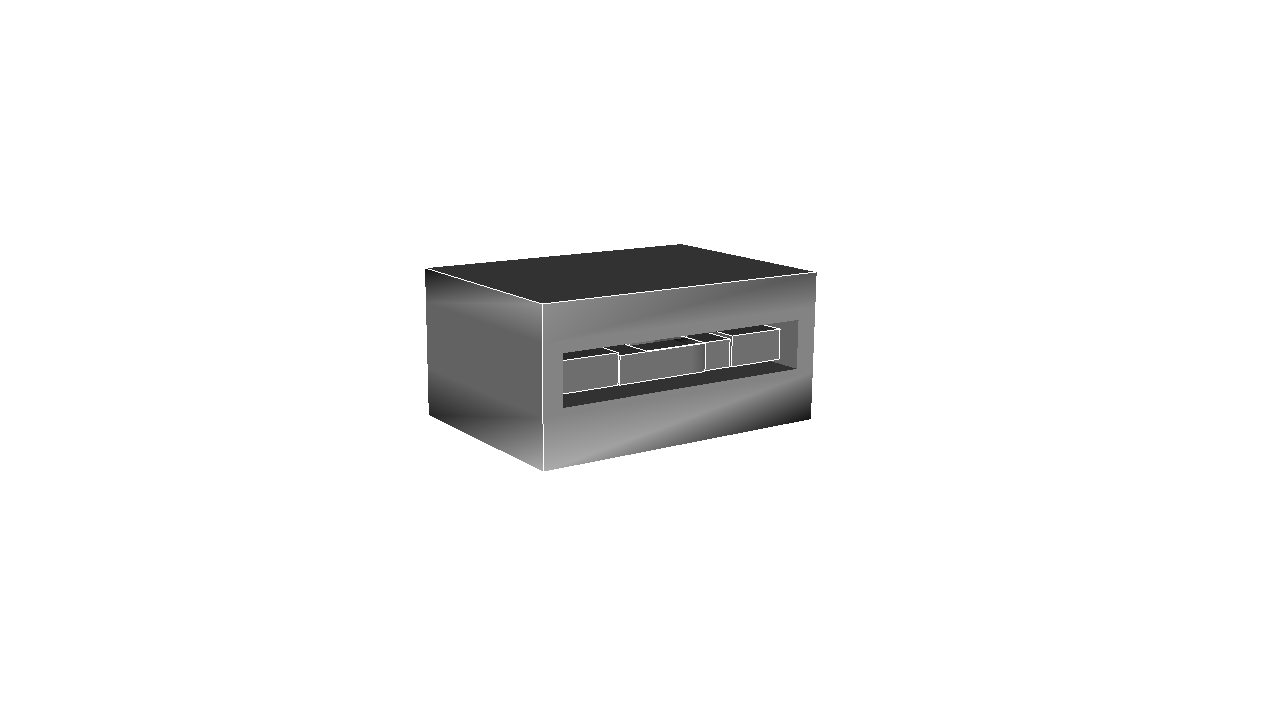
\includegraphics[width=0.5\linewidth]{img/caps/test10_1.png}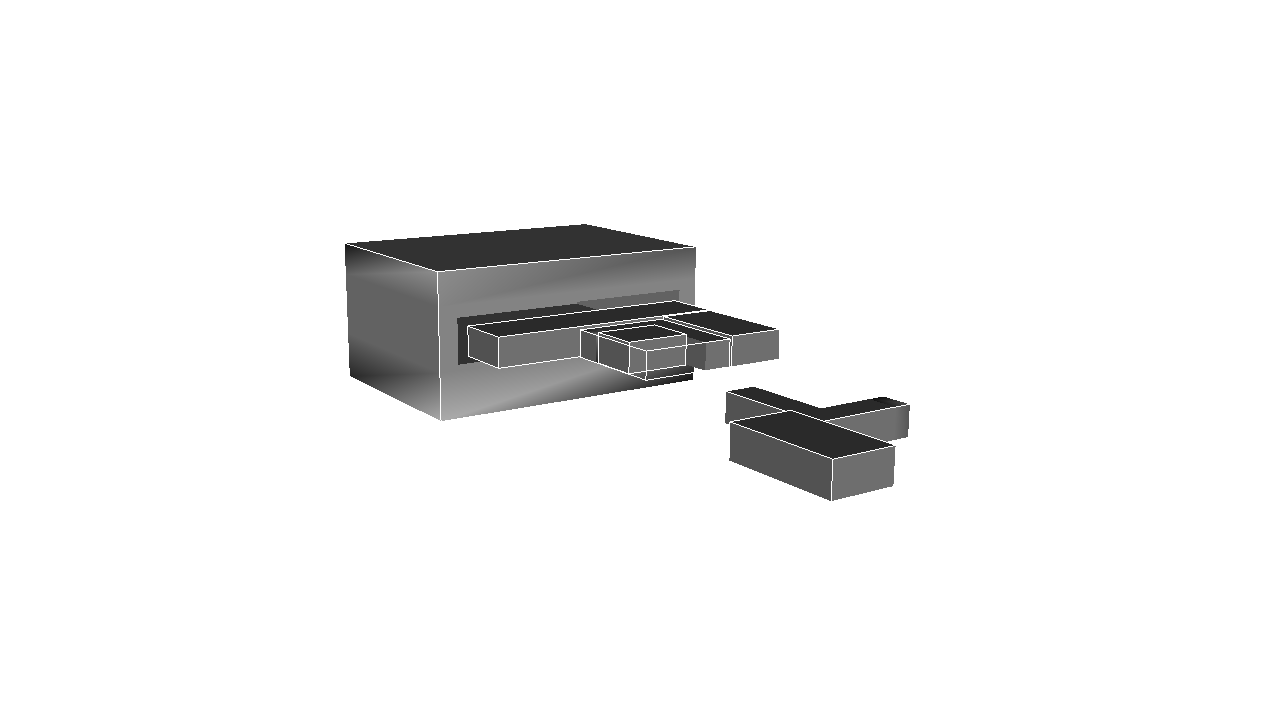
\includegraphics[width=0.5\linewidth]{img/caps/test10_2.png}}
	\caption{\label{fig:test10} Modelo 6 antes e depois da explos�o da parte central.}
\end{figure*}